\documentclass[10pt]{ctexart}
\usepackage{listings}
\usepackage{amsmath} 
\usepackage{amssymb} 
\usepackage{xcolor}
\usepackage{xeCJK}
\usepackage{fontspec}
\usepackage{titlesec}
\usepackage{titletoc}
\usepackage{setspace}
\usepackage{graphicx}
\usepackage{geometry}
\usepackage[T1]{fontenc}  
\usepackage{textcomp}
\usepackage{lmodern}
%\usepackage{caption}
\usepackage[justification=centering]{subcaption}
\usepackage[justification=centering]{caption}
\usepackage{tikz}
\usetikzlibrary{graphs}
\usepackage{amsfonts}
\usepackage[colorlinks,
            linkcolor=black,
            anchorcolor=black,
            citecolor=black]{hyperref}
\geometry{a4paper,scale=0.8}
\renewcommand\contentsname{Contents}
%\setmonofont[Mapping={}]{Monaco}    %英文引号之类的正常显示,相当于设置英文字体
%\setsansfont{Consolas} %设置英文字体 Monaco, Consolas,  Fantasque Sans Mono
%\setmainfont{Monaco} %设置英文字体
\setmonofont{Consolas}
% 定义可能使用到的颜色
%\setmainfont[BoldFont=SimHei]{SimSun}
\definecolor{CPPLight}  {HTML} {686868}
\definecolor{CPPSteel}  {HTML} {888888}
\definecolor{CPPDark}   {HTML} {262626}
\definecolor{CPPBlue}   {HTML} {4172A3}
\definecolor{CPPGreen}  {HTML} {487818}
\definecolor{CPPBrown}  {HTML} {A07040}
\definecolor{CPPRed}    {HTML} {AD4D3A}
\definecolor{CPPViolet} {HTML} {7040A0}
\definecolor{CPPGray}  {HTML} {B8B8B8}
\lstset{
    columns=fixed,       
    % numbers=left,                                        % 在左侧显示行号
    frame=none,                                          % 不显示背景边框
    backgroundcolor=\color[RGB]{245,245,244},            % 设定背景颜色
    keywordstyle=\color[RGB]{40,40,255},                 % 设定关键字颜色
    numberstyle=\small\color{darkgray},                  % 设定行号格式
    commentstyle=\it\color[RGB]{0,96,96},                % 设置代码注释的格式
    stringstyle=\rmfamily\slshape\color[RGB]{128,0,0},   % 设置字符串格式
    showstringspaces=false,                              % 不显示字符串中的空格
    language=c++,                                        % 设置语言
    morekeywords={alignas,continute,friend,register,true,alignof,decltype,goto,
    reinterpret_cast,try,asm,defult,if,return,typedef,auto,delete,inline,short,
    typeid,bool,do,int,signed,typename,break,double,long,sizeof,union,case,
    dynamic_cast,mutable,static,unsigned,catch,else,namespace,static_assert,using,
    char,enum,new,static_cast,virtual,char16_t,char32_t,explict,noexcept,struct,
    void,export,nullptr,switch,volatile,class,extern,operator,template,wchar_t,
    const,false,private,this,while,constexpr,float,protected,thread_local,
    const_cast,for,public,throw,std},
    emph={map,set,multimap,multiset,unordered_map,unordered_set,
    unordered_multiset,unordered_multimap,vector,string,list,deque,
    array,stack,forwared_list,iostream,memory,shared_ptr,unique_ptr,
    random,bitset,ostream,istream,cout,cin,endl,move,default_random_engine,
    uniform_int_distribution,iterator,algorithm,functional,bing,numeric,},
    emphstyle=\color{CPPViolet},
    basicstyle=\linespread{1}\small\fontspec{Consolas}\ttfamily,
    breaklines=true,
    %xleftmargin=1em,xrightmargin=1em, aboveskip=1em,
    % in the listings package configuration, try:  
    literate={"}{\textquotedbl}1,  
    tabsize=4, keepspaces=true
}
\CTEXoptions[today=old]
\title{Exercises 6}
\author{软件工程一班 \ 张逸松 57号}
\date{\today}

\begin{document}
    \maketitle
    \subsection*{7.4}
    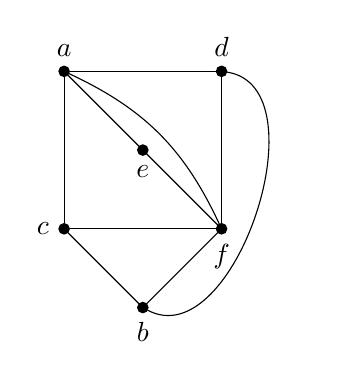
\begin{tikzpicture}
        \node (c) at (0, 0) [circle , draw, fill = black, label = left :$c$, scale = 0.4pt] {};
        \node (a) at (0, 2) [circle , draw, fill = black, label = above:$a$, scale = 0.4pt] {};
        \node (f) at (2, 0) [circle , draw, fill = black, label = below:$f$, scale = 0.4pt] {};
        \node (d) at (2, 2) [circle , draw, fill = black, label = above:$d$, scale = 0.4pt] {};
        \node (e) at (1, 1) [circle , draw, fill = black, label = below:$e$, scale = 0.4pt] {};
        \node (b) at (1, -1) [circle , draw, fill = black, label = below:$b$, scale = 0.4pt] {};
        \draw [] (a) edge (c);
        \draw [] (c) edge (f);
        \draw [] (f) edge (d);
        \draw [] (d) edge (a);
        \draw [] (a) edge (e);
        \draw [] (e) edge (f);
        \draw [bend left = 20] (a) edge (f);
        \draw [] (c) edge (b);
        \draw [] (f) edge (b);
        \draw [bend right = 100] (b) edge (d);
    \end{tikzpicture}
    \subsection*{7.5} It is nonplanar.
    \subsection*{7.10}
    \begin{itemize}
        \item [\textbf{a)}] It becomes to a $K_4$, is planar.
        \item [\textbf{b)}] It becomes to a $K_5$, is nonplanar.
        \item [\textbf{c)}] It becomes to a $K_{2,3}$, is planar.
        \item [\textbf{d)}] It becomes to a $K_{2,4}$, is planar.
    \end{itemize}
    \subsection*{7.13}
    It contains a subgraph homeomorphic to $K_5$, so it is nonplanar.
\end{document}